\documentclass{article}
\usepackage{amsmath,amsfonts,bm}
\usepackage{tikz}
\usetikzlibrary{positioning, shapes, arrows, fit, backgrounds}

\begin{document}

    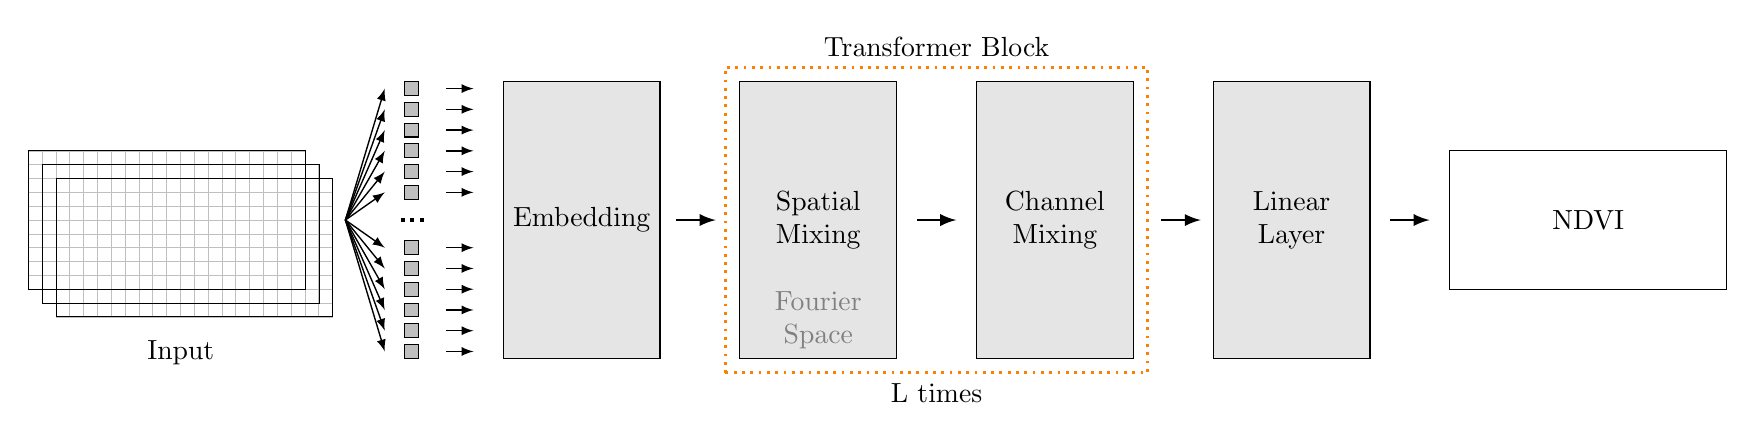
\begin{tikzpicture}[
  node distance=1cm,
  >=latex,
]

  % Leftmost block (Embedding)
  \node[draw=black, fill=gray!20, rectangle, minimum height=10em, minimum width=3em, text width=5em, align=center] (embedding) at (0,0) {Embedding};

  % Draw the vertical line of rectangles and dotted points
  \foreach \i in {1,...,6} {
    %Boxes
    \draw[fill=gray!50] (-2.25cm, {(\i-1)*0.75em - 5em}) rectangle +(0.5em, 0.5em);
    \draw[fill=gray!50] (-2.25cm, {(\i-1)*0.75em + 0.75em}) rectangle +(0.5em, 0.5em);

    %Arrows from Boxes to Embedding
    \draw[-latex, line width = 0.5pt] (-2.25cm + 1.5em, {(\i-1)*0.75em - 4.75em}) -- ++(0.35, 0);
    \draw[-latex, line width = 0.5pt] (-2.25cm + 1.5em, {(\i-1)*0.75em + 1em}) -- ++(0.35, 0);

    %Arrows from input to Boxes
    \draw[-latex, line width = 0.5pt] (-3cm , 0 ) -- (-2.5cm ,{(\i-1)*0.75em - 4.75em});
    \draw[-latex, line width = 0.5pt] (-3cm , 0 ) -- (-2.5cm ,{(\i-1)*0.75em + 1em});
   }
   \draw[dotted, line width=1.5pt] (-2.3cm,-0em) -- (-2cm,-0em);

 % Define the input node
  \node[draw=black, rectangle, minimum height=5em, minimum width=10em, align=center, left=2.5cm of embedding] (input1) {};

  \node[draw=black, rectangle, minimum height=5em, minimum width=10em, align=center, left=2.5cm of embedding, shift={(0.5em,-0.5em)}] (input2) {};

  \node[draw=black, rectangle, minimum height=5em, minimum width=10em, align=center, left=2.5cm of embedding, shift={(1em,-1em)}] (input3) {};

  \node[below=1em] at (input2.south) {Input};


  % Draw grid lines behind the inputs
  \begin{scope}[on background layer]
    \draw[step=0.5em, gray!50, very thin, align=center] (input1.south west) grid (input1.north east);
    \draw[step=0.5em, gray!50, very thin, align=center] (input2.south west) grid (input2.north east);
    \draw[step=0.5em, gray!50, very thin, align=center] (input3.south west) grid (input3.north east);    
  \end{scope}


  % Spatial
  \node[draw=black, fill=gray!20, rectangle, minimum height=10em, minimum width=3em, right=of embedding, text width=5em, align=center] (spatmix)  {Spatial \\ Mixing};
  \node[above, text width=5em, align=center, text=black!50] at (spatmix.south) {Fourier Space};

  % Channel Mixing block
  \node[draw=black, fill=gray!20, rectangle, minimum height=10em, minimum width=3em, text width=5em, align=center, right=of spatmix] (chanmix) {Channel \\ Mixing};

  % Linear block
  \node[draw=black, fill=gray!20, rectangle, minimum height=10em, minimum width=3em, text width=5em, align=center, right=of chanmix] (linear) {Linear \\ Layer};

  % NDVI block
  \node[draw=black, rectangle, minimum height=5em, minimum width=10em, align=center, right=of linear] (ndvi) {NDVI};


  \node[draw=orange, dotted, line width=1pt, fit=(spatmix) (chanmix), inner sep=0.5em] (dottedrect) {};
  \node[below] at (dottedrect.south) {L times};
  \node[above] at (dottedrect.north) {Transformer Block};


  % % Arrow between Blocks
  \draw[-latex, line width = 1pt] (embedding.east) ++(0.20,0) -- ++(0.5, 0);
  \draw[-latex, line width = 1pt] (spatmix.east) ++(0.25,0) -- ++(0.5, 0);
  \draw[-latex, line width = 1pt] (chanmix.east) ++(0.35,0) -- ++(0.5, 0);
  \draw[-latex, line width = 1pt] (linear.east) ++(0.25,0) -- ++(0.5, 0);

\end{tikzpicture}

\end{document}